% L6b student companion deck.
%
% The frame order mirrors the lecture notebook so students can take notes while
% the instructor works through the notebook. The disclaimer is intentionally
% slide 2, by instructor preference.
\documentclass[aspectratio=169,11pt]{beamer}
\usepackage{vnslides}

\newcommand{\E}{\mathbb{E}}
\newcommand{\Var}{\operatorname{Var}}
\newcommand{\Cov}{\operatorname{Cov}}
\newcommand{\bg}{\mathbf{g}}
\newcommand{\bw}{\mathbf{w}}
\newcommand{\br}{\mathbf{r}}
\newcommand{\bal}{\boldsymbol{\alpha}}
\newcommand{\bbe}{\boldsymbol{\beta}}
\newcommand{\beps}{\boldsymbol{\varepsilon}}
\newcommand{\Dg}{\mathbf{D}_{g}}
\newcommand{\Sig}{\boldsymbol{\Sigma}_{g}}
\newcommand{\SigSIM}{\hat{\boldsymbol{\Sigma}}_{g,\mathrm{SIM}}}
\newcommand{\gSIM}{\hat{\bg}_{\mathrm{SIM}}}
\newcommand{\Tan}{\mathcal{T}}
\newcommand{\np}{|\mathcal P|}

\title{\texorpdfstring{{\vnheavy L6b}}{L6b}: Single Index Model Portfolio Allocation}
\subtitle{CHEME 5660 Cornell University}
\author{Copyright Jeffrey Varner 2026. All Rights Reserved}

\begin{document}

\vntitlepage

\begin{frame}{Disclaimer and Risks}
  \vspace{0.6em}
  \textbf{\ink{Training only.}} This content is for training and informational
  purposes only. The teaching team does not make, give, or endorse any offer or
  solicitation to buy or sell securities or derivative products, or provide
  investment or trading advice or strategy.

  \vspace{1.1em}
  \textbf{\ink{Risk.}} Trading involves risk and is generally not recommended for
  those with limited resources, experience, or a low risk tolerance. Past
  performance does not guarantee future success.

  \vspace{1.1em}
  \textbf{\ink{Responsibility.}} You are responsible for your investment decisions
  based on your financial circumstances, objectives, risk tolerance, and
  liquidity needs.
\end{frame}

\begin{frame}{Objectives for Today}
  Today we put the single index model of L6a to work: assemble its inputs for a
  portfolio, solve L5b's allocation problems with them, and compare the result
  with the data-driven portfolios in sample and out of sample.

  \vspace{0.6em}
  {\large\textbf{\ink{Today's concepts}}}
  \vspace{0.2em}
  \begin{itemize}\setlength{\itemsep}{0.45em}
    \item \hilite{Construct and diagnose SIM portfolio inputs}: the SIM mean
      vector and covariance from the archive, why the mean vector reproduces the
      sample means, and which residual covariances the SIM omits.
    \item \hilite{Solve SIM allocation problems}: long-only risky and risky and
      risk-free portfolios, the tangent portfolio from the ray of solutions, and
      what bounds, a borrowing restriction, or a higher borrowing rate change.
    \item \hilite{Evaluate what the model changes}: weights and covariance regret
      in sample, frozen allocations on the 2025 test year, and what one split can
      and cannot say.
  \end{itemize}
\end{frame}

\begin{frame}{Lectures and Examples}
  \vspace{0.3em}
  {\normalsize\textbf{\ink{Lecture:}}\par
  \dimmed{CHEME-5660-L6b-Lecture-SIM-Portfolio-RF-Fall-2026.ipynb}}

  \vspace{0.7em}
  {\normalsize\textbf{\ink{Example 1:}}\par
  \dimmed{CHEME-5660-L6b-Example-SIM-MinVar-RA-Fall-2026.ipynb}}

  \vspace{0.7em}
  {\normalsize\textbf{\ink{Example 2:}}\par
  \dimmed{CHEME-5660-L6b-Example-SIM-MinVar-RRFA-Fall-2026.ipynb}}

  \vspace{0.6em}
  The first example assembles the SIM inputs for thirteen firms, checks two exact
  facts about them, traces the long-only frontier from each input set, compares
  weights and regret, and scores the portfolios on 2025 data. The second adds
  the risk-free asset, reads the tangent portfolio off the ray of solutions, and
  scores complete portfolios that lend, hold, or borrow.
\end{frame}

% ==== concept review =========================================
\begin{frame}{Concept Review: The Single Index Model and Its Covariance}
  L6a: for asset $i\in\mathcal P$ on day $t$, with growth rate $g_{i,t}$ (inverse
  years), market growth rate $g_{M,t}$ (SPY; $M$ names the index), intercept
  $\alpha_i$, exposure $\beta_i$, and residual $\varepsilon_{i,t}$:
  \[
    g_{i,t}=\alpha_i+\beta_i\,g_{M,t}+\varepsilon_{i,t}
  \]
  with $\E[\varepsilon_{i,t}]=0$, $\Cov(\varepsilon_{i,t},g_{M,t})=0$, and
  $\Cov(\varepsilon_{i,t},\varepsilon_{j,t})=0$ for $i\ne j$.
  Stack the assets ($\bg,\bal,\bbe,\beps$), let $\bar g_M=\E[g_M]$,
  $\sigma^2_{g,M}=\Var(g_M)$, and
  $\Dg=\operatorname{diag}(\sigma^2_{g,\varepsilon,1},\ldots,\sigma^2_{g,\varepsilon,\np})$;
  under the three assumptions:
  \[
    \boxed{\bar{\bg}=\bal+\bbe\,\bar g_M,\qquad
      \Sig=\sigma^2_{g,M}\,\bbe\bbe^{\top}+\Dg}
  \]
  \hilite{Rank one plus diagonal}: $2\np+1$ numbers for the covariance and
  $\np+1$ for the mean, in place of $\np(\np+1)/2$ covariances. Uncorrelated
  residuals is the assumption that makes it a covariance model.
\end{frame}

\begin{frame}{Concept Review: Portfolio Risk and the Archive}
  For fixed weights $\bw$, the linearized growth rate $g_p=\bw^{\top}\bg$ (L5b)
  has portfolio beta $\beta_p=\bw^{\top}\bbe$ and:
  \[
    \Var(g_p)=\underbrace{\beta_p^2\,\sigma^2_{g,M}}_{\text{market risk}}
      +\underbrace{\bw^{\top}\Dg\bw}_{\text{residual risk}}
  \]

  \vspace{0.1em}
  \begin{itemize}\setlength{\itemsep}{0.35em}
    \item Everything above is a population statement.
    \item The L6a estimation example fitted the model by least squares for every
      security in the 2014 to 2024 data and saved the estimates: that archive is
      where today's inputs come from.
    \item \hilite{Derivation} (one line): $g_i-\E[g_i]=\beta_i(g_M-\bar g_M)+\varepsilon_i$;
      multiply for $i,j$, take expectations; the assumptions kill the cross
      terms and, for $i\ne j$, the residual product.
  \end{itemize}
  \slidenote{Catch-up:}{\dimmed{../L6a/CHEME-5660-L6a-Example-SVD-SIM-Estimation-Fall-2026.ipynb}}
\end{frame}

% ==== inputs from the archive ================================
\begin{frame}{SIM Portfolio Inputs from the Archive}
  The archive holds, per security fitted against SPY on the $N$ training days,
  the least-squares estimates $\hat\alpha_i$, $\hat\beta_i$, and the residual
  variance $s^2_{g,\varepsilon,i}=\lVert\br_i\rVert_2^2/(N-2)$ ($\br_i$ the
  fitted residual series), and once the training-period sample mean $g'_M$ and
  variance $s^2_{g,M}$ of the market. Substituting estimates for population
  quantities gives the SIM inputs for a portfolio:
  \[
    \boxed{\gSIM=\hat{\bal}+\hat{\bbe}\,g'_M,\qquad
      \SigSIM=s^2_{g,M}\,\hat{\bbe}\hat{\bbe}^{\top}+\hat{\Dg},\qquad
      \hat{\Dg}=\operatorname{diag}(s^2_{g,\varepsilon,1},\ldots,s^2_{g,\varepsilon,\np})}
  \]

  \vspace{0.2em}
  \begin{itemize}\setlength{\itemsep}{0.45em}
    \item \hilite{Market moments from the training period}: taking them from a
      later window mixes an in-sample fit with out-of-sample information; the
      archive stores the training values so it cannot happen by accident.
    \item Growth-rate units throughout: means in inverse years, variances in
      inverse years squared, no $\Delta t$ (L6a).
  \end{itemize}
\end{frame}

\begin{frame}{Two Exact Facts about the SIM Inputs}
  How do they compare with L5b's data-driven inputs, the sample means
  $\hat{\bg}$ and sample covariance $\hat{\Sig}$ of the same firms over the same
  days?

  \vspace{0.4em}
  \hilite{The SIM mean vector is the sample-mean vector.} A least-squares line
  with an intercept passes through the point of sample means (the residuals sum
  to zero), so $\hat\alpha_i+\hat\beta_i g'_M=g'_i$ and
  $\gSIM=\hat{\bg}$. The two input sets agree on the reward.

  \vspace{0.4em}
  \hilite{The SIM covariance is the sample covariance with the residual
  covariances removed.} Residuals are orthogonal to the ones and to the market
  series, so:
  \[
    \hat\Sigma_{g,ij}=\hat\beta_i\hat\beta_j\,s^2_{g,M}+\widehat{\Cov}(\br_i,\br_j)
  \]
  so off the diagonal $(\hat{\Sig}-\SigSIM)_{ij}=\widehat{\Cov}(\br_i,\br_j)$
  exactly, the residual covariances L6a measured; on the diagonal only $N-1$
  versus $N-2$ on the residual term, $-\lVert\br_i\rVert_2^2/[(N-1)(N-2)]$, a
  factor of about $1.0004$.
\end{frame}

\begin{frame}{Where the SIM Covariance Errs, and Positive Definiteness}
  The SIM covariance error is not a vague approximation: it is the residual
  covariance, pair by pair, with the sign structure L6a found.
  \begin{itemize}\setlength{\itemsep}{0.4em}
    \item Same industry: positively correlated residuals (banks with banks by
      several tenths; automakers; semiconductor firms). The SIM
      \hilite{understates} their correlation.
    \item Technology firms with banks: negatively correlated residuals, two or
      three tenths. The SIM \hilite{overstates} their correlation.
    \item The SIM correlation matrix has one pattern, off the diagonal
      $\hat\beta_i\hat\beta_j s^2_{g,M}$ over the two total standard deviations,
      so no blocks; the data have blocks.
  \end{itemize}

  \vspace{0.3em}
  \hilite{Positive definiteness}: for any $\mathbf x$,
  $\mathbf x^{\top}\SigSIM\mathbf x=s^2_{g,M}(\hat{\bbe}^{\top}\mathbf x)^2+\sum_i s^2_{g,\varepsilon,i}x_i^2\ge0$;
  positive definite whenever every residual variance is positive (sufficient,
  not necessary). It is what the closed forms need; it says nothing about
  whether the matrix describes future co-movement.
\end{frame}

% ==== risky-only =============================================
\begin{frame}{Risky Asset Portfolios using Single Index Models}
  L5b's long-only problem with SIM inputs, for a target growth rate $g_\star$:
  \[
    \boxed{\begin{aligned}
      \min_{\bw}\ &\bw^{\top}\SigSIM\bw
        =\underbrace{s^2_{g,M}(\hat{\bbe}^{\top}\bw)^2}_{\text{market risk}}
        +\underbrace{\textstyle\sum_i s^2_{g,\varepsilon,i}w_i^2}_{\text{residual risk}}\\
      \text{s.t.}\ &\gSIM^{\top}\bw\ge g_\star,\qquad \mathbf 1^{\top}\bw=1,\qquad 0\le w_i\le1
    \end{aligned}}
  \]

  \vspace{0.2em}
  \begin{itemize}\setlength{\itemsep}{0.45em}
    \item Market term depends on the weights only through the portfolio beta;
      the residual term is a weighted sum of squares that diversification
      shrinks.
    \item The target is a floor: sweeping $g_\star$ from the GMV growth rate
      upward traces the GMV portfolio and the efficient branch, same convex
      quadratic program, same package.
  \end{itemize}
\end{frame}

\begin{frame}{Same Means, Different Covariance: Regret}
  The mean vectors agree, so \hilite{every difference between the two frontiers
  is a residual covariance}. For the same weights (ordered pairs):
  \[
    \bw^{\top}\SigSIM\bw=\bw^{\top}\hat{\Sig}\bw
      -\sum_{i\ne j}w_iw_j\,\widehat{\Cov}(\br_i,\br_j)
      +\sum_i\frac{\lVert\br_i\rVert_2^2}{(N-1)(N-2)}\,w_i^2
  \]
  The SIM \hilite{understates} variance where the held residuals correlate
  positively and \hilite{overstates} it where they correlate negatively. The
  honest comparison evaluates the SIM weights under the data covariance at the
  same target: the \hilite{regret}
  $\bw_{\mathrm{SIM}}(g_\star)^{\top}\hat{\Sig}\,\bw_{\mathrm{SIM}}(g_\star)-\bw(g_\star)^{\top}\hat{\Sig}\,\bw(g_\star)\ge0$,
  because the data-optimal weights minimize exactly that quantity. Example 1: a
  variance regret of $0.01$ to $1.2$, a gap of a few thousandths to a tenth of a
  standard-deviation unit; nearly the same firms, weights up to seven points apart.
  \slidenote{Example 1:}{\dimmed{CHEME-5660-L6b-Example-SIM-MinVar-RA-Fall-2026.ipynb}}
\end{frame}

% ==== risky + risk-free ======================================
\begin{frame}{Risky and Risk-Free Asset Portfolios using Single Index Models}
  Add L5b's risk-free asset: growth rate $g_f$, zero variance over the matched
  horizon (a bill or a STRIP held to maturity; sold earlier it carries L2b's
  rate risk). Risk-free fraction $w_f$, risky weights $\bw$, $w_f+\mathbf 1^{\top}\bw=1$.
  The problem the package solves:
  \[
    \boxed{\min_{\bw}\ \bw^{\top}\SigSIM\bw\quad\text{s.t.}\quad
      \gSIM^{\top}\bw+\underbrace{(1-\mathbf 1^{\top}\bw)}_{w_f}\,g_f\ge g_\star,\qquad
      0\le w_i\le1}
  \]

  \vspace{0.2em}
  \begin{itemize}\setlength{\itemsep}{0.45em}
    \item Only the risky weights carry variance and only they are bounded;
      \hilite{$w_f$ is not sign-constrained}: $w_f<0$ borrows at $g_f$, and the
      package allows it.
    \item Eliminating $w_f$: a constraint on the \hilite{excess} growth rate,
      $(\gSIM-g_f\mathbf 1)^{\top}\bw\ge g_\star-g_f$.
  \end{itemize}
\end{frame}

\begin{frame}{The Solutions Lie on a Ray}
  Scale the risky weights by a positive constant: excess growth scales by it,
  variance by its square, $w_i\ge0$ unchanged. So, for feasible $g_\star>g_f$
  ($\SigSIM\succ0$, so the minimizer is unique) and until an upper bound
  $w_i\le1$ binds, the minimizers are \hilite{one risky direction} scaled by the target. With $\bw_{\Tan}$ the point on the ray with
  $\mathbf 1^{\top}\bw=1$ ($w_f=0$):
  \[
    \boxed{\bw(g_\star)=(1-w_f)\,\bw_{\Tan},\qquad
      1-w_f=\frac{g_\star-g_f}{\E[g_{\Tan}]-g_f}}
  \]

  \vspace{0.2em}
  \begin{itemize}\setlength{\itemsep}{0.4em}
    \item Below $\E[g_{\Tan}]$: lend ($0<w_f<1$). Above: borrow ($w_f<0$). Valid
      until $(1-w_f)\max_i w_{\Tan,i}=1$, then the boundary kinks.
    \item $\bw_{\Tan}=\bw/\mathbf 1^{\top}\bw$ from \hilite{any} solution on the
      ray (at $g_\star=g_f$ the solution is $\mathbf 0$).
    \item Example 2 sweeps the target, checks every normalized solution is the
      same vector, and reads $\bw_{\Tan}$ off the ray: the tangent portfolio of
      L5b.
  \end{itemize}
\end{frame}

\begin{frame}{The Picture}
  \begin{center}
    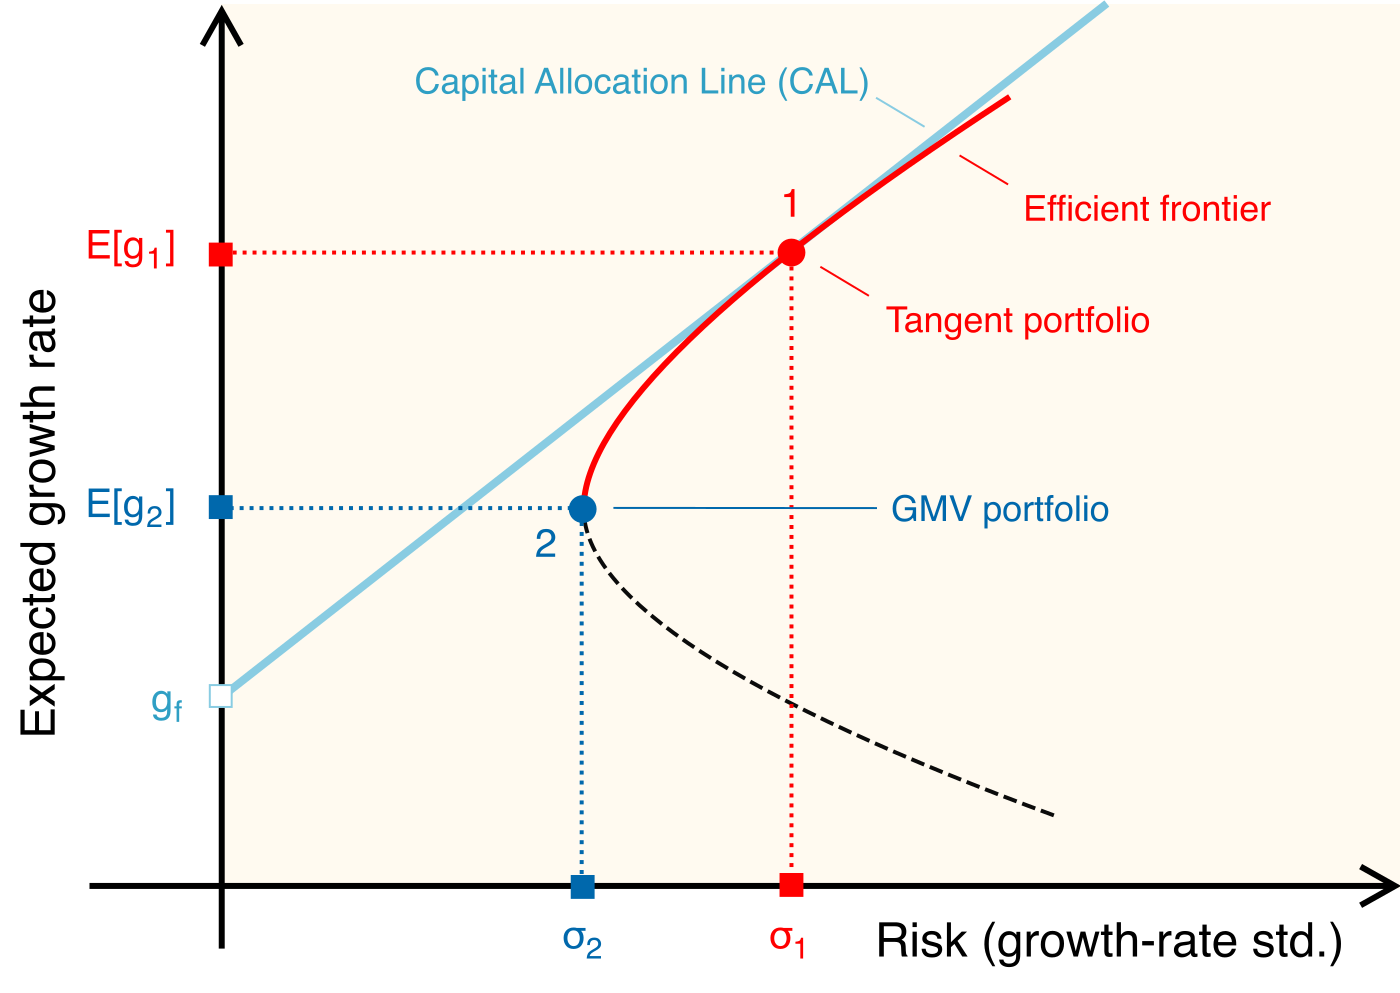
\includegraphics[height=0.62\textheight,keepaspectratio]{../figs/Fig-MinVar-RiskFree-Schematic.png}
  \end{center}
  \vspace{-0.4em}
  Portfolio 1 is the tangent portfolio $\Tan$, portfolio 2 the GMV portfolio;
  the CAL runs from $(0,g_f)$ through $\Tan$; the dashed lower branch is
  dominated.
\end{frame}

\begin{frame}{The Capital Allocation Line and the Tangent Portfolio (Recall)}
  L5b: mixing a risky portfolio $p$ ($\E[g_p]$, $\sigma_{g,p}>0$) with fraction
  $w_f$ risk-free gives $\E[g_c]=g_f+(1-w_f)(\E[g_p]-g_f)$ and
  $\sigma_{g,c}=|1-w_f|\,\sigma_{g,p}$; eliminating $w_f$ (for $w_f\le1$) gives
  the \hilite{capital allocation line} $\E[g_c]=g_f+\mathrm{SR}_p\,\sigma_{g,c}$,
  a line from $(0,g_f)$ through $p$ whose slope is the Sharpe ratio
  $\mathrm{SR}_p=(\E[g_p]-g_f)/\sigma_{g,p}$.
  \begin{itemize}\setlength{\itemsep}{0.4em}
    \item A steeper line is better at every risk: hold the risky portfolio with
      the largest Sharpe ratio, the \hilite{tangent portfolio} $\Tan$; its CAL
      touches the frontier at $\Tan$.
    \item The ray \hilite{is} that CAL: least variance per unit of excess growth
      is the largest Sharpe ratio, so the ray's direction is the long-only
      maximum-Sharpe portfolio (Example 2 checks it against the frontier).
    \item Under SIM inputs, with $\hat\beta_{\Tan}=\hat{\bbe}^{\top}\bw_{\Tan}$:
      $\mathrm{SR}_{\Tan}=\bigl(\hat{\bal}^{\top}\bw_{\Tan}+\hat\beta_{\Tan} g'_M-g_f\bigr)\big/
      \sqrt{s^2_{g,M}\hat\beta_{\Tan}^2+\bw_{\Tan}^{\top}\hat{\Dg}\bw_{\Tan}}$.
  \end{itemize}
\end{frame}

\begin{frame}{Closed Form and Sharpe Conventions (Recall)}
  \begin{itemize}\setlength{\itemsep}{0.55em}
    \item \hilite{Closed form} (shorts allowed, $\SigSIM\succ0$, GMV portfolio
      earns more than $g_f$): $\bw_{\Tan}\propto\SigSIM^{-1}(\gSIM-g_f\mathbf 1)$
      normalized to sum to one; the rank-one-plus-diagonal structure gives the
      inverse in closed form (notes). Long-only: no closed form; the ray or the
      frontier sweep.
    \item \hilite{Which Sharpe ratio}: with $\sigma_{g,p}$ in the denominator it
      is the CAL slope in growth-rate units, a one-observation-interval quantity.
      Dividing by the volatility $\sqrt{\Delta t}\,\sigma_{g,p}$ ($\Delta t$ the
      observation interval in years) gives the
      \hilite{annualized} value $\mathrm{SR}_p/\sqrt{\Delta t}$, larger by
      $\sqrt{252}\approx15.9$. Same ranking; from here on the course quotes
      annualized.
    \item Example 2: about $1.3$ annualized for both the SIM and the data-driven
      tangent portfolios on the training data; both hold the same three
      high-growth technology names, the SIM version less concentrated plus a
      small semiconductor position.
  \end{itemize}
\end{frame}

\begin{frame}{Separation, and What Breaks It}
  $\Tan$'s CAL dominates every other, so all mean-variance investors sharing
  estimates, $g_f$, horizon, and opportunity set hold one risky fund and differ only in $w_f$
  (Tobin, L5b): exact with one rate and no constraints; survives the long-only
  constraint on the risky weights. What breaks it:
  \begin{itemize}\setlength{\itemsep}{0.15em}
    \item \hilite{No borrowing} ($w_f\ge0$): truncates the straight CAL segment
      at $\Tan$; above it the efficient boundary generally returns to the risky
      frontier, so separation holds only piecewise. Not imposed by the package.
    \item \hilite{Position bounds} ($w_i\le1$, or a concentration limit
      $w_i\le u$): kink the ray where they bind. Imposed in practice because
      unconstrained maximum-Sharpe portfolios put extreme weights on a few assets
      when the means are imprecise; a lower in-sample Sharpe, maybe more robust.
    \item \hilite{Borrowing rate above the lending rate}: kinks the line at $\Tan$.
  \end{itemize}
  \slidenote{Example 2:}{\dimmed{CHEME-5660-L6b-Example-SIM-MinVar-RRFA-Fall-2026.ipynb}}
\end{frame}

% ==== what changes, how to check =============================
\begin{frame}{What the SIM Inputs Change, and How to Check}
  \begin{itemize}\setlength{\itemsep}{0.5em}
    \item The SIM does \hilite{not} change the reward input; it replaces the
      sample covariance by a rank-one-plus-diagonal matrix that omits the
      residual covariances, with $2\np+1$ numbers instead of $\np(\np+1)/2$.
    \item Where most residual correlations are small (median $0.14$ here, a few
      industry pairs $0.6$ to $0.7$) that costs little in sample: nearly the same
      assets, weights up to seven points apart, a standard-deviation gap of at
      most a tenth. It bites for two banks or two share classes of one firm.
    \item What it buys is not visible with thirteen firms: with hundreds of
      assets and a few years of daily data the sample covariance has more
      parameters than the data pin down and its inverse amplifies noise (L5b
      advanced); the SIM covariance is a few numbers per asset, always
      positive semidefinite, interpretable. Whether that helps out of sample is
      an empirical question about the universe.
  \end{itemize}
\end{frame}

\begin{frame}{Checking: Freeze, Test, Read for What It Is}
  \begin{itemize}\setlength{\itemsep}{0.5em}
    \item \hilite{Freeze} everything on the training window: universe, SIM
      parameters, market moments, $g_f$ at the decision date, weights.
    \item \hilite{Test} the frozen weights with the buy-and-hold wealth rule on
      the test year, next to baselines: equal weights, the GMV portfolio, an
      index fund.
    \item \hilite{Read} it as one year, one draw, one universe. The paired SIM
      and data-driven portfolios earned nearly the same 2025 wealth: the input
      sets selected nearly the same portfolios, and one year cannot rank them
      (the gap is far smaller than the sampling error). Realized risk of the
      complete portfolios scaled almost exactly with $1-w_f$ (buy-and-hold
      drifts, so not exactly);
      realized growth did not match the model, whose least certain input is the
      tangent portfolio's growth.
    \item Narrow beta intervals do not imply stable weights: propagating L6a's
      parameter uncertainty into the weights is the advanced notebook, and the
      question to ask before trading.
  \end{itemize}
\end{frame}

% ==== optional advanced material =============================
\begin{frame}{Optional Advanced Material}
  \vspace{0.4em}
  {\normalsize\textbf{\ink{Advanced:}} \dimmed{advanced/uncertainty/}\par
  \dimmed{CHEME-5660-L6b-Advanced-SIM-Portfolio-Uncertainty-Fall-2026.ipynb}}

  \vspace{0.7em}
  Optional, not a prerequisite for L7a. Bootstraps the SIM parameters of a
  six-firm universe two ways (empirical residuals and Gaussian innovations),
  keeps each asset's joint draw of intercept, beta, and residual scale, rebuilds
  the SIM covariance for every draw, and reads the distributions of a fixed
  unconstrained minimum-variance portfolio's growth-rate standard deviation, allocation
  distance, and variance regret.
  \slidenote{Notebook:}{\href{https://github.com/varnerlab/CHEME-5660-CourseRepository-Fall-2026/tree/main/lectures/week-6/L6b/advanced}{lectures/week-6/L6b/advanced}, also linked from the lecture notebook.}
\end{frame}

\begin{frame}{Summary}
  Today: the SIM inputs for a portfolio, L5b's allocation problems with them,
  the CAL and separation as the package computes them, and the comparison in
  and out of sample.

  \vspace{0.1em}
  {\large\textbf{\ink{Key takeaways}}}
  \vspace{0.05em}
  \begin{itemize}\setlength{\itemsep}{0.2em}
    \item \hilite{The SIM changes only the covariance, and we know how}: same
      sample means; sample covariance minus the off-diagonal residual covariances.
    \item \hilite{One risky answer for every risk-free fraction}: a free $w_f$
      makes the constraint one on excess growth, every target scales one
      direction by $1-w_f$, and the fully invested point is the tangent portfolio;
      bounds, no borrowing, or a higher borrowing rate kink or truncate the ray.
    \item \hilite{Regret in sample, frozen weights out of sample}: SIM weights
      under the data covariance can only lose, and by little here; one test year
      checks weights without ranking input sets.
  \end{itemize}
  Next, L7a: a utility-based rebalancing engine, preferences recomputed daily.
\end{frame}

\transitionframe{Today: the same means, a covariance you can write the error of, and one risky answer for every risk-free fraction.}

\end{document}
